\documentclass[12pt,twoside,openright]{report} 
\usepackage{mathtools}
\usepackage{bm}
\usepackage{isomath}
\usepackage{verbatim}
\usepackage{upgreek}

%load any additional packages
%\usepackage{amssymb}
\usepackage{graphicx,color}
\usepackage{natbib}
\setcitestyle{citesep={;}, aysep={,}, yysep={,}}

\graphicspath{{./figures/}}

\setlength{\topmargin}{0.0in}
\setlength{\oddsidemargin}{0.33in}
\setlength{\evensidemargin}{-0.08in}
\setlength{\textheight}{8.5in}
\setlength{\textwidth}{6.0in}

%input macros (i.e. write your own macros file called mymacros.tex 
%and uncomment the next line)
%\include{mymacros}

\newcommand{\bs}[1]{\boldsymbol{#1}}
\newcommand{\wrong}[1]{(\textcolor{red}{not #1})}
\newcommand\emptypage{
\newpage
\thispagestyle{empty}
\mbox{}
\newpage
}

\def\mytitle{Thesis title long title very long title indeed a long title so long that it goes to next line}
\def\myname{Mech. Student A and Mech. Student B}
\def\mydegree{Degree Title}
\def\mysupervisor{Mech Supervisor}
\def\myrollno{00ME10001 and 00ME10002}
\def\mydep{Mechanical Engineering}
\def\mydegreedate{Month 20xx}


%end the preamble and start the document
\begin{document}

%this baselineskip gives sufficient line spacing for an examiner to easily
%markup the thesis with comments
\baselineskip=18pt plus1pt

%set the number of sectioning levels that get number and appear in the contents
\setcounter{secnumdepth}{3}
\setcounter{tocdepth}{3}


%\maketitle                  % create a title page from the preamble info
         % include the abstract

\pagenumbering{roman}
\thispagestyle{empty}
\begin{center}
    { \large {\bfseries {\mytitle}} \par}
\vspace{3\baselineskip}
    {\textit{Thesis submitted to the} \\ \textit{Indian Institute of Technology Kharagpur} \\ \textit{In partial fulfillment for the award of the degree} \par}
\vspace{\baselineskip}
    {\textit{of} \par}
\vspace{\baselineskip}
    {\large \bf \mydegree \par} 
\vspace{\baselineskip}
    {\textit{by} \par}
\vspace{\baselineskip}
    {{\large {\bf \myname \\ \myrollno}} \par}
%\vspace{-0.1\baselineskip}
%    {{\large {\bf \myrollno}} \par}
\vspace{1.5\baselineskip}
    {Under the guidance of \par}
\vspace{\baselineskip}
    {{\large \bf \mysupervisor} \par}
\vspace{1.5\baselineskip}
    {\begin{figure}[!h] 
	\centering
	
\includegraphics[width=32mm]{./iitkgplogo.JPG} 
     \end{figure}
    }
%{\large \vspace*{1ex}
%\vspace{\baselineskip}
    {\bf \MakeUppercase{\mydep} \par}
\vspace*{1ex}
    {\bf \uppercase{Indian Institute of Technology Kharagpur} \par}
%\vspace*{25mm}
%    {{\submittedtext} \par}
%\vspace*{2ex}
    {\Large \mydegreedate \par}
    {\copyright $\,$\myname. All rights reserved.}
  \end{center}


%\maketitle
%\begin{dedication}
This thesis is dedicated to\\
 someone\\
for some special reason\\
\end{dedication}        % include a dedication.tex file
\emptypage
\addcontentsline{toc}{chapter}{Certificate}
\begin{center}
{\Large {\bf \uppercase{Certificate}}}
\end{center}
\thispagestyle{plain}
\noindent This is to certify that the thesis entitled {\bf \mytitle}, submitted by {\bf \myname} to the Indian Institute of Technology Kharagpur, is a record of bona fide research work under my supervision and I consider it worthy of consideration for the award of the degree of {\bf \mydegree} of the Institute. 
\vspace{3\baselineskip}
\begin{flushright}
\begin{minipage}[c]{0.4\textwidth}
\centering
\hrule 
\vspace{0.5\baselineskip}
{\Large \bf Supervisor} \\
\end{minipage}
\end{flushright}
\vspace{\baselineskip}

{\large \bf Date: }

\emptypage
\addcontentsline{toc}{chapter}{Declaration}
\begin{center}
{\Large {\bf \uppercase{Declaration}}}
\end{center}
\thispagestyle{plain}
\noindent I certify that 
%\vspace{1\baselineskip}

\begin{itemize}
\item[a.] The work contained in the thesis is original and has been done by myself under the general supervision of my supervisor.
\item[b.] The work has not been submitted to any other Institute for any degree or diploma. 
\item[c.] I have followed the guidelines provided by the Institute in writing the thesis. 
\item[d.] I have conformed to the norms and guidelines in the Ethical Code of Conduct of the Institute. 
\item[e.] Whenever I have used materials (data, theoretical analysis, and text) from other sources, I have given due credit to them by citing them in the text of the thesis and giving their details in the references. 
\item[f.] Whenever I have quoted written materials from other sources, I have put them under quotation marks and given due credit to the sources by citing them and giving required details in the references. 
\end{itemize}

\begin{flushright}
\begin{minipage}[c]{0.5\textwidth}
%\centering
%\hrule 
\vspace{3\baselineskip}
{\large \bf Signature of the Student} \\
\end{minipage}
\end{flushright}

\vspace{\baselineskip}

%{\large \bf Date: }

\emptypage
\addcontentsline{toc}{chapter}{Acknowledgements}
\thispagestyle{plain}
\begin{center}
{\Large \bf \uppercase{Acknowledgements}}
\end{center}
plenty of waffle, plenty of waffle, plenty of waffle, plenty of waffle,
plenty of waffle, plenty of waffle, plenty of waffle, plenty of waffle.

   
\emptypage
\addcontentsline{toc}{chapter}{List of Symbols and Abbreviations}
\begin{center}
{\Large \bf \uppercase{List of Symbols and Abbreviations}}
\end{center}
 
\emptypage
\addcontentsline{toc}{chapter}{Abstract}
\begin{center}
{\Large \bf \uppercase{Abstract}}
\end{center}
plenty of waffle, plenty of waffle, plenty of waffle, plenty of waffle,
plenty of waffle, plenty of waffle, plenty of waffle, plenty of waffle.
 

%\begin{romanpages}          % start roman page numbering
\tableofcontents            % generate and include a table of contents
%\listoffigures              % generate and include a list of figures
%\end{romanpages}            % end roman page numbering


\clearpage


\pagenumbering{arabic}
%now include the files of latex for each of the chapters etc
\chapter{Sample Title}

Lorem ipsum dolor sit amet, consectetur adipiscing elit, sed do eiusmod tempor incididunt ut labore et dolore magna aliqua. Ut enim ad minim veniam, quis nostrud exercitation ullamco laboris nisi ut aliquip ex ea commodo consequat. Duis aute irure dolor in reprehenderit in voluptate velit esse cillum dolore eu fugiat nulla pariatur. Excepteur sint occaecat cupidatat non proident, sunt in culpa qui officia deserunt mollit anim id est laborum.

\section{On Referencing}


%One of the biggest sources of irritation to anyone evaluating a report is the inconsistent use of citation and referencing style. The higher the irritation induced, the more easily are the marks deducted! 
The whole business of referencing has two components to it: the citations within the text and the list of references at the end.

\subsection{Citations within the text}
When you wish to cite a particular reference that you have used to do your research, you have at your disposal various citation styles: the numerical style, the author-year style, the author-number style, and so on. Far too often, I have seen that while at one place in the report, the numerical style of citation, like [1], is used to refer to a paper, at another place in the report, the author-year style is used, like \citep{2013JMPSCui}. At IIT Kharagpur, the recommended style is a particular flavour of the author-year style called the Harvard style.\footnote{Actually, what IIT Kharagpur prescribes is a slight variation on top of the Harvard style.}  \\

A citation to a reference in the author-year style can appear in two primary ways within the text:
\begin{itemize}
\item The names of the authors form part of the sentence. 
\item The names of the authors do not form part of a sntence.
\end{itemize}

In the following, some important points regarding these two ways of citation, as recommended by IIT Kharagpur, are mentioned:

\subsubsection{Author names form part of the sentence}

In certain sentences you will need to include the names of the author(s) in the sentence itself. For example
\begin{quote} 
``The theory of special relativity was proposed by \citet{Einstein3}." 
\end{quote}


There are some finer points involved here:

\begin{itemize}
\item Use ONLY the surname of authors. \textcolor{red}{Do NOT use the full name or abbreviated name. The following are wrong:}
\begin{quote}
\textcolor{red}{``A. Einstein (1905) proposed the theory of special relativity."}\\
\textcolor{red}{``The influence of surface mechanics was investigated by Yang-Tse Cheng and M. Verbrugge (2008)."}
\end{quote} 

\item For certain sentence constructions, you will need to respect the singular or plural sense. If there is only author, use the singular verb. If there are multiple authors, use the plural verb. 
\begin{quote}
``\citet{Einstein3} was responsible for proposing the theory of special relativity." \\
``\citet{2008ChengVerbrugge} have investigated the influence of surface mechanics."
\end{quote}


\item If there are three or more authors, use the first author's surname followed by {\em et~al.} For example:
\begin{quote}
``\citet{2013JMPSCui} have studied the influence of interface-reaction on lithium diffusion in silicon." 
\end{quote}

\item If the same author or group of authors have multiple papers, then the following citation style must be used:
\begin{quote}
``The influence of surface mechanics has been investigated by \citet{2008ChengVerbrugge, 2009ChengVerbrugge}."
\end{quote}
Notice, in the above, that the different years are separated by comma. The years MUST be in chronological order.

\item If the same author or group of authors have multiple papers in the same year, the the following citation style must be used:
\begin{quote}
``Two important structural issues in cylindrical anode particles were investigated by \citet{2015IJSSChakraborty, 2015JPSChakraborty}."
\end{quote}


\end{itemize}

%\clearpage

\subsubsection{Author names do not form part of the sentence}


If the sentence you are writing is such that it just needs to be supported by a reference, the citation must be placed within parentheses. For example:
\begin{quote}
``An entire field of research was opened in physics by the proposition of the theory of relativity \citep{Einstein3}." 
\end{quote}

Some finer points are described below:

\begin{itemize}
\item Notice, in the above example, that there is a comma between the surname and the year. 

\item Again, ONLY the surnames of author(s) must be used. 

\item Notice, again in the above example, that even if the citation is removed, the sentence is grammatically correct and makes complete sense. It is a major point of difference from the previous style where the names of the authors were part of the sentence. 

\item \textcolor{red}{The following examples are NOT correct:}
\begin{quote}
\textcolor{red}{``An entirely new field of physics was opened by \citep{Einstein3}."} \\
\textcolor{red}{``The paper by \citep{Einstein3} opened an entirely new field of physics."}
\end{quote}

\item It is not necessary that the citation be placed at the end of the sentence. A citation may appear at any appropriate place within the sentence. There may be multiple sets of references spread throughout the sentence. For example:
\begin{quote}
``Various facets associated with diffusion-induced stresses have been studied ranging from surface mechanics \citep{2008ChengVerbrugge}, buckling \citep{2015IJSSChakraborty}, and length increase \citep{2015JPSChakraborty}."
\end{quote}


\item If you need to put more than one reference within parentheses, use semi-colons to separate them. For example:
\begin{quote}
``Mathematical models of silicon anodes in lithium-ion batteries have included various features like diffusion-induced stress and stress-influenced diffusion \citep{2008ChengVerbrugge, 2013JMPSCui}."
\end{quote}
\end{itemize}

\vspace{0.5cm}

\noindent {\bf VERY IMPORTANT:} Overall, every reference that is cited within the text must correspondingly appear in the Reference list at the end. Conversely, every reference appearing in the Reference list must have been cited at least once somewhere in the text. 

\subsection{List of References}

Please go through the list of References at the end of this document very carefully and note the following sequence of items:
\begin{itemize}
\item The surnames appear first, followed by the initials. 
\item The names are followed by the year of publication (within brackets). 
\item Then the title of the paper appears within single quotes. Capital letters should not be arbitrarily sprinkled within the title. Capital letters MUST be used where necessary; for example, ``Li-ion battery". 
\item The next item is the name of the journal (in italics) where appropriate capitalization has been used. Not every word is capitalized. For example, ``of", ``the", ``and" are in small letters.  
\item The journal name is followed by the volume number in bold. 
\item Finally, the page numbers appear. Certain journals assign only an article number instead of page numbers. 
\end{itemize}

The sequence described above with proper punctuations and formatting MUST be maintained uniformly across all references.  


\begin{figure}[!htb]
\centering
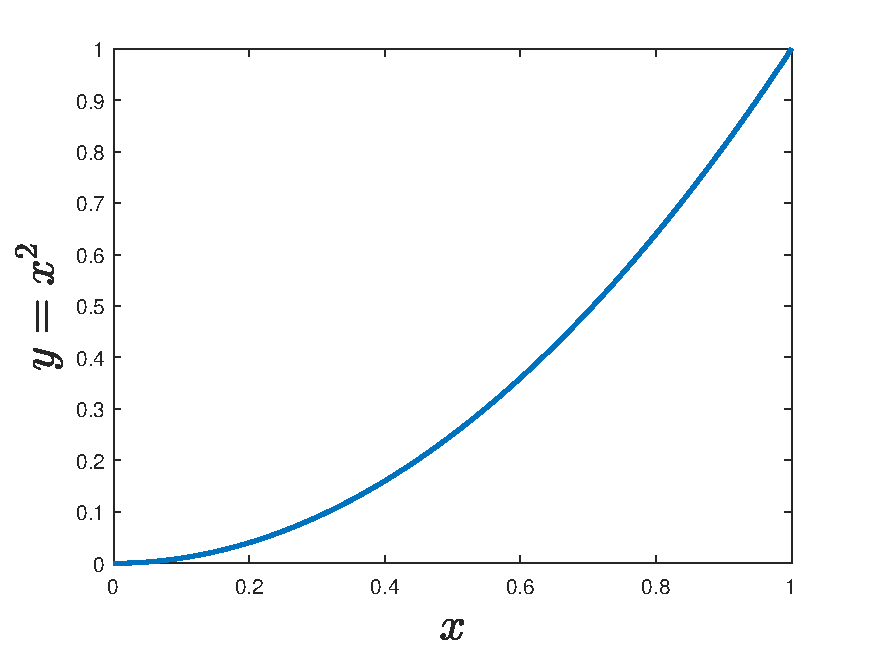
\includegraphics[width=0.5\textwidth]{./ch1_figs/trial.pdf}
\end{figure}



\chapter{Sample Title}

Lorem ipsum dolor sit amet, consectetur adipiscing elit, sed do eiusmod tempor incididunt ut labore et dolore magna aliqua. Ut enim ad minim veniam, quis nostrud exercitation ullamco laboris nisi ut aliquip ex ea commodo consequat. Duis aute irure dolor in reprehenderit in voluptate velit esse cillum dolore eu fugiat nulla pariatur. Excepteur sint occaecat cupidatat non proident, sunt in culpa qui officia deserunt mollit anim id est laborum.
\chapter{Summary and Conclusions}

Lorem ipsum dolor sit amet, consectetur adipiscing elit, sed do eiusmod tempor incididunt ut labore et dolore magna aliqua. Ut enim ad minim veniam, quis nostrud exercitation ullamco laboris nisi ut aliquip ex ea commodo consequat. Duis aute irure dolor in reprehenderit in voluptate velit esse cillum dolore eu fugiat nulla pariatur. Excepteur sint occaecat cupidatat non proident, sunt in culpa qui officia deserunt mollit anim id est laborum.


%now enable appendix numbering format and include any appendices
\appendix
\chapter{Sample Title}

Lorem ipsum dolor sit amet, consectetur adipiscing elit, sed do eiusmod tempor incididunt ut labore et dolore magna aliqua. Ut enim ad minim veniam, quis nostrud exercitation ullamco laboris nisi ut aliquip ex ea commodo consequat. Duis aute irure dolor in reprehenderit in voluptate velit esse cillum dolore eu fugiat nulla pariatur. Excepteur sint occaecat cupidatat non proident, sunt in culpa qui officia deserunt mollit anim id est laborum.
\chapter{Sample Title}

Lorem ipsum dolor sit amet, consectetur adipiscing elit, sed do eiusmod tempor incididunt ut labore et dolore magna aliqua. Ut enim ad minim veniam, quis nostrud exercitation ullamco laboris nisi ut aliquip ex ea commodo consequat. Duis aute irure dolor in reprehenderit in voluptate velit esse cillum dolore eu fugiat nulla pariatur. Excepteur sint occaecat cupidatat non proident, sunt in culpa qui officia deserunt mollit anim id est laborum.

%next line adds the Bibliography to the contents page
\addcontentsline{toc}{chapter}{References}
%uncomment next line to change bibliography name to references
%\renewcommand{\bibname}{References}
\bibliographystyle{agsm}  %use the plain bibliography style
\bibliography{refs}        %use a bibtex bibliography file refs.bib

\end{document}

